\documentclass[12pt]{article}%
\usepackage{amsfonts}
\usepackage{fancyhdr}
\usepackage{comment}
\usepackage[a4paper, top=2.5cm, bottom=2.5cm, left=2.2cm, right=2.2cm]%
{geometry}
\usepackage{times}
\usepackage{amsmath}
\usepackage{changepage}
\usepackage{amssymb}
\usepackage{graphicx}%
\setcounter{MaxMatrixCols}{30}
\newtheorem{theorem}{Theorem}
\newtheorem{acknowledgement}[theorem]{Acknowledgement}
\newtheorem{algorithm}[theorem]{Algorithm}
\newtheorem{axiom}{Axiom}
\newtheorem{case}[theorem]{Case}
\newtheorem{claim}[theorem]{Claim}
\newtheorem{conclusion}[theorem]{Conclusion}
\newtheorem{condition}[theorem]{Condition}
\newtheorem{conjecture}[theorem]{Conjecture}
\newtheorem{corollary}[theorem]{Corollary}
\newtheorem{criterion}[theorem]{Criterion}
\newtheorem{definition}[theorem]{Definition}
\newtheorem{example}[theorem]{Example}
\newtheorem{exercise}[theorem]{Exercise}
\newtheorem{lemma}[theorem]{Lemma}
\newtheorem{notation}[theorem]{Notation}
\newtheorem{problem}[theorem]{Problem}
\newtheorem{proposition}[theorem]{Proposition}
\newtheorem{remark}[theorem]{Remark}
\newtheorem{solution}[theorem]{Solution}
\newtheorem{summary}[theorem]{Summary}
\newenvironment{proof}[1][Proof]{\textbf{#1.} }{\ \rule{0.5em}{0.5em}}

\newcommand{\Q}{\mathbb{Q}}
\newcommand{\R}{\mathbb{R}}
\newcommand{\C}{\mathbb{C}}
\newcommand{\Z}{\mathbb{Z}}

\begin{document}

\title{Homework 1}
\author{Weijia Zhan}
\date{\today}
\maketitle

\section{Problem 1}
\subsection{Accuracy}
\subsubsection{backward-Euler}
\begin{equation} \label{eq1}
\begin{split}
\frac{\psi(t_{n}) - \psi(t_{n} - \Delta t)}{\Delta t}  & = \frac{d\psi}{dt}(t_{n}) \\
\end{split}
\end{equation}



Expand $\psi(t_{n} - \Delta t)$ at $t_{n}$,
\begin{equation} \label{eq2}
\begin{split}
\psi(t_{n} - \Delta t) & = \psi(t_{n}) - \Delta t\frac{d\psi}{dt}(t_{n}) + \frac{(-\Delta t)^{2}}{2}\frac{(d^{2}\psi)}{dt^{2}}(t_{n}) + \frac{(-\Delta t)^{3}}{6}\frac{d^{3}\psi}{dt^{3}}(t_{n})  + ... \\
\end{split}
\end{equation}

Substitute equation \ref{eq2} into equation \ref{eq1},
\begin{equation} \label{eq3}
\begin{split}
\frac{\psi(t_{n}) - \psi(t_{n} - \Delta t)}{\Delta t}  - \frac{d\psi}{dt}(t_{n}) &= -\frac{(\Delta t)}{2}\frac{(d^{2}\psi)}{dt^{2}}(t_{n}) + \frac{(\Delta t)^{2}}{6}\frac{d^{3}\psi}{dt^{3}}(t_{n})  + ... \\
\end{split}
\end{equation}

This lowest order of $\Delta t$ on the RHS of equation \ref{eq3} is 1, the accuracy of backward differencing scheme is first-order accuracy.

\subsubsection{trapezoidal}
\begin{equation} \label{eq4}
\begin{split}
\frac{\psi(t_{n}+\Delta t) - \psi(t_{n})}{\Delta t}  = \frac{1}{2}(\frac{d\psi}{dt}(t_{n}+ \Delta t) + \frac{d\psi}{dt}(t_{n}) )
\end{split}
\end{equation}
The truncation error is,
\begin{equation} \label{eq5}
\begin{split}
&\frac{\psi(t_{n} + \Delta t) - \psi(t_{n})}{\Delta t} - \frac{1}{2}(\frac{d\psi}{dt}(t_{n} + \Delta t)+ \frac{d\psi(t_{n})}{dt})\\
& = \frac{d\psi(t_{n})}{dt} + \frac{(\Delta t)}{2}\frac{(d^{2}\psi)}{dt^{2}}(t_{n}) + \frac{(\Delta t)^{2}}{6}\frac{d^{3}\psi}{dt^{3}}(t_{n})  + ... \\
&- \frac{1}{2}(2\frac{d\psi}{dt}(t_{n}) + \Delta t\frac{(d^{2}\psi)}{dt^{2}}(t_{n}) + \frac{(\Delta t)^{2}}{2}\frac{d^{3}\psi}{dt^{3}}(t_{n})  + ...)\\
& = -\frac{(\Delta t)^{2}}{12}\frac{d^{3}\psi}{dt^{3}}(t_{n}) + O((\Delta t)^{3})
\end{split}
\end{equation}
Then the accuracy is second-order accuracy.
\subsection{A-stability}
\subsubsection{backward-Euler}
As, 
\begin{equation} \label{eq6}
\begin{split}
\frac{\psi_{n} - \psi_{n-1}}{\Delta t}  = \frac{d\psi_{n}}{dt} = (\lambda + iw)\psi_{n}
\end{split}
\end{equation}
then,
\begin{equation} \label{eq7}
\begin{split}
\frac{\psi_{n}}{\psi_{n-1}} = \frac{1}{1 - \lambda \Delta t - iw\Delta t} 
\end{split}
\end{equation}
thus,
set A = $|\frac{\psi_{n}}{\psi_{n-1}}| \leq 1$,
\begin{equation} \label{eq8}
\begin{split}
&A = |\frac{\psi_{n}}{\psi_{n-1}}| = |\frac{1}{1 - \lambda \Delta t - iw\Delta t} | \leq 1\\
& |1 - \lambda \Delta t - iw\Delta t| \geq 1 \\
&(1 - \lambda \Delta t)^{2} + (w\Delta t)^{2} \geq 1
\end{split}
\end{equation}
This equation is just for the area outside of the circle centered at $(\lambda \Delta t, 0)$ with radius of 1, so backward Euler is A-stable. 
\subsubsection{trapezoidal}

\begin{equation} \label{eq9}
\begin{split}
&\frac{\psi_{n+1} - \psi_{n}}{\Delta t}  = \frac{1}{2}(\frac{d\psi_{n+1}}{dt} + \frac{d\psi_{n}}{dt}) \\
& = \frac{1}{2}(\gamma\psi_{n+1} + \gamma\psi_{n})\\
& \rightarrow |\frac{\psi_{n+1}}{\psi_{n}}| = |\frac{1 + \frac{\gamma \Delta t}{2} + }{1 - \frac{\gamma \Delta t}{2}}| 
\end{split}
\end{equation}
set $A =  |\frac{\psi_{n+1}}{\psi_{n}}| \leq 1$,
equation \ref{eq9} becomes,
\begin{equation} \label{eq10}
\begin{split}
&|A| = |\frac{1+\frac{\lambda \Delta t}{2} + \frac{iw\Delta t}{2}}{1 - \frac{\lambda \Delta t}{2} -\frac{iw\Delta t}{2}}| \leq 1 \\
& |A^{2}| = \frac{(1 + \frac{\lambda \Delta t}{2})^{2} + (w\Delta t)^{2}}{(1 - \frac{\lambda \Delta t}{2})^{2} + (w\Delta t)^{2}} \leq 1
\end{split}
\end{equation}
This implies that $\lambda\Delta t \leq 0$, which is the half plane of the coordinate system, so trapezoidal method is A-stable.

\section{Problem 2}
See Figure \ref{fig:fig1}.
\begin{figure}
    \centering
    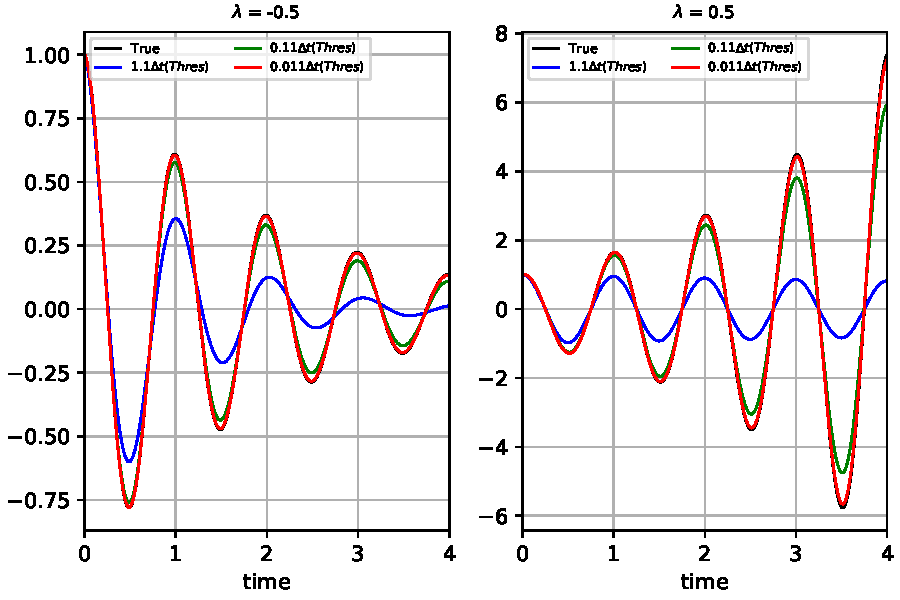
\includegraphics{figs/backward.pdf}
    \caption{Backward-Euler scheme.}
    \label{fig:fig1}
\end{figure}


\section{Problem 3}
See Figure \ref{fig:fig2}.
\begin{figure}
    \centering
    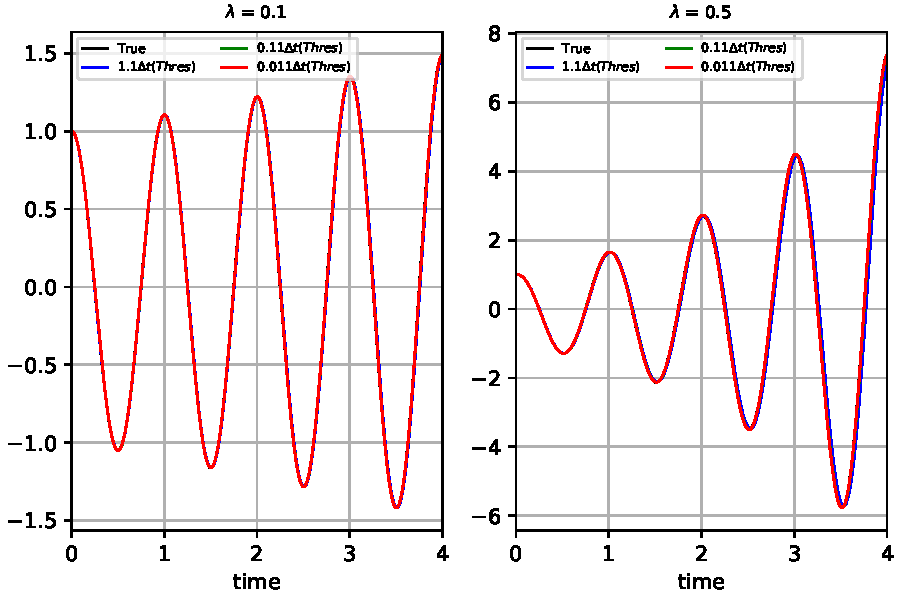
\includegraphics{figs/trapezoidal.pdf}
    \caption{Trapezoidal method.}
    \label{fig:fig2}
\end{figure}
\section{Problem 4}


When checking the numerical results of three different schemes, the main differences are as follows:

1.With different lengths of time step, the amplification of amplitudes are different among each other. Forward scheme method tends to amplify the magnitude with time going on and are sensitive to length of the time step. Backward-Euler scheme method tends to reduce the magnitude with time going on and is also sensitive to time. Trapezoidal method is not sensitive to time.

2. The shifts in time (falling behind or not) are different using different $\lambda$. When $\lambda$ is negative (positive), the amplitudes of the solutions show no (increasing) shift in time using Forward scheme and  show increasing (no) shift in time using Backward-Euler scheme with increasing length of time step. With increasing $\lambda$, solution using Trapezoidal method tends to shit in time with increasing length of time step.

\end{document}